\documentclass[a4paper,11pt,dvipdfmx]{ujarticle}
% パッケージ
\usepackage{graphicx}
\usepackage{url}
% レイアウト指定を記述したファイルの読み込み
\input{layout}

\title{日本におけるデジタル化の状況}
\author{G684262026 鵜飼純之介}

\begin{document}

\maketitle 

\section{デジタル競争力ランキング}
国際経営開発研究所（IMD）の調査\cite{imd}によると,日本のデジタル競争力
のランキングは図\ref{fig:fig31}に示すように,調査対象の64カ国中,
総合で28位,知識分野で25位となっている.

\begin{figure}[htbp]
    \centering
    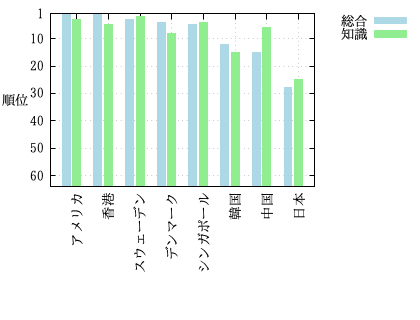
\includegraphics{fig31.png}
    \caption{デジタル競争力ランキング(64カ国中)}
    \label{fig:fig31}
\end{figure}

\newpage

\section{ブローバンドの整備状況}
OECDによりブロードバンド回線の普及に関する調査\cite{oecd}によると,
表\ref{tab:tab1}に示すように,
日本における100人あたりのブロードバンド加入者数は190.5で,
第1位になっている.2位はエストニアで,3位は米国と続く

\begin{table}[htbp]
    \centering
    \caption{モバイルブロードバンドの加入者数（100人あたり）}
    \label{tab:tab1}
    \begin{tabular}{|c|c|c|}
        \hline
        順位 & 国名 & 加入者数 \\
        \hline
        1位 & 日本 & 190.5 \\
        \hline
        2位 & エストニア & 179.9 \\
        \hline
        3位 & 米国 & 169.0 \\
        \hline
        4位 & フィンランド & 157.0 \\
        \hline
        5位 & デンマーク & 141.7 \\
        \hline
        6位 & ラトビア & 141.6 \\
        \hline
        7位 & イスラエル & 139.9 \\
        \hline
        8位 & オランダ & 133.7 \\
        \hline
        9位 & ポーランド & 131.3 \\
        \hline
        10位 & スウェーデン & 127.2 \\
        \hline
    \end{tabular}
\end{table}

\section{考察}
\begin{itemize}
    \item 日本は図\ref{fig:fig31}のデジタル競争力ランキングにおいてはそこまで高い順位ではないが,表\ref{tab:tab1}より,ブロードバンド回線の普及は進んでいることから,インターネット回線などへの知識がないままインターネット回線を使う人が多いことがわかる.
    \item 図\ref{fig:fig31}では上位にすら入っていないエストニアが,表\ref{tab:tab1}では2位に入っていることから,エストニアでは上記の傾向がより顕著であると考えられる.
\end{itemize}


\bibliographystyle{junsrt}
\bibliography{exercise.bib}

\end{document}